\documentclass[conference]{IEEEtran}
\usepackage{amsmath,amssymb,amsfonts}
\usepackage{url}
\usepackage{subfigure}
\usepackage{booktabs,threeparttable,multirow}

\usepackage{graphicx}
\graphicspath{{images/}}

% new math operators
\DeclareMathOperator{\abs}{abs}

% todo command
\usepackage{marginnote}
\newcounter{todocnt}
\newcommand{\Sim}{\textsc{Simon}} 
\setcounter{todocnt}{0}
\newcommand{\todo}[1]{\stepcounter{todocnt}{\tt {[#1]}} \marginpar{{$\blacksquare$ \thetodocnt}}}  
\newcommand{\specialcell}[2][c]{%
  \begin{tabular}[#1]{@{}c@{}}#2\end{tabular}}

\hyphenation{op-tical net-works semi-conduc-tor}
\IEEEoverridecommandlockouts
\begin{document}

\title{Integrated Power Analysis Platform}


\author{\IEEEauthorblockN{Tuan Vu
}
\IEEEauthorblockA{Worcester Polytechnic Institute, 
Worcester, MA 01609, USA\\
Email: \texttt{quangvu@wpi.edu}
}}
\maketitle

\begin{abstract}
Power analysis of a embedded cryptographic device often require a high sampling rate of power consumption at high resolution. The quality of captured data directly contributes to the effectiveness of power analysis attacks. High-speed and high-resolution data acquisition capability does not come cheap however; often require a high-powered oscilloscope. Additionally, a typical data acquisition setup is complicated, involving multiple stages of capturing and processing data. The goal of this project is to offer an affordable and integrated alternative to the typical setup by using the BeagleBone Black embedded Linux platform and custom data acquisition hardware extension.
\end{abstract}

\section{Motivation}\label{sec:motivation}
There is a reason why oscilloscopes cost as much as they do: high-speed and high-resolution data acquisition is difficult to achieve. A general-purpose Tektronix base model oscilloscope can cost more than \$1000 and high-end model can cost upward of \$19000 in the Tektronix 5054B model case.

Replacing an expensive data acquisition setup with an affordable and integrated alternative is therefore desirable. This project poses the question: Can an inexpensive piece of equipment offer the same data resolution and sampling rate as a high-powered oscilloscope? It cannot; but it may be able to achieve the same end result.

\section{Background}\label{sec:background}
As mentioned in section \ref{sec:motivation}, ensuring the quality of captured data using inexpensive alternative setup is the main obstacle that this project is attempting to overcome. 

The first step is therefore to establish the minimum requirement for a "usable" set of data; in other words, what is the minimum sampling rate and resolution needed for a successful power analysis attack?

\subsection{Nyquist Theorem}
The famous Nyquist theorem \cite{nyquist1928certain}, a.k.a. sampling theorem, states that the optimal sampling rate of any signal is twice its maximum frequency. Oversampling yields no significant improvement on accuracy, while undersampling loses signal fidelity. The theorem has therefore revealed an upper bound on the required sampling rate for any signal as described in equation \ref{eq:nyquist}.

\begin{equation}\label{eq:nyquist}
f^{*}_{sampling} = 2*f_{signal_max}
\end{equation}

Modern RISC microprocessor typically operate in the Megahertz range; for example, the targeted ATMega328p runs at 8MHz. Applying Nyquist theorem gives the optimal sampling rate of 16MHz for accurate signal reconstruction.

\subsection{Microprocessor Architecture}
Another important factor in determining the optimal sampling rate is the microarchitecture of the intended target. The targeted microprocessor may run in the Megahertz range but it is simply means how fast the clock is running. A more accurate measurement of a microprocessor's performance is the number of instructions per second being executed; the unit for this measurement is Million Instruction Per Second (MIPS).

The targeted ATMega328p has the following architectural characteristics that reduces its maximum MIPS:

\subsubsection{8-bit architecture} drastically reduces the performance of frequently used operations such as multiplication and division when compared to a 32-bit microprocessor (e.g. ARM). The effect is especially noticeable during RSA encryption/decryption operations. For AES, there should be virtually no difference in performance since all operations are byte-oriented.

\subsubsection{Two-stage pipeline} a design technique to optimize CPU excecution throughput: instructions are fetched then executed. While most of the instruction set executes in only one (1) clock cycle, the multiplication instruction takes two (2) cycle for the execution phase, which reduces MIPS count.

\subsection{Captured Data Resolution}
In telecommunication theory, the Shannon-Hartley theorem \cite{shannon1949communication} shows a relationship between the maximum signal bandwidth/frequency that can be transmitted over a channel and the observed noise level. The smaller the noise, or conversely the larger the Signal-to-Noise (SNR) ratio, the higher signal bandwidth/frequency one can send. The maximum theoretical limit is called the Nyquist rate which is twice the bandwidth of the channel. Basically, this theorem states that there is a minimum SNR required to allow sampling the signal at the optimal Nyquist sampling rate.

In practice, it is rather complicated to accurately predict the minimal sampling resolution needed to distinguish signal noise from actual variation in power consumption using this theorem. Unfortunately, this means adjustment has to be made on a case-by-case basis.

\subsection{Related Works}
The most recent relevant work is a correlation-based power analysis attack done on an ATMega328p microprocessor running an AES-128 implementation at 16MHz by Banerjee, Ho and Skoppula~\cite{Banerjee2015}.

The report states that a Tektronix 5054B computing oscilloscope model was critical for a successful attack. According to the technical specification, the aforementioned oscilloscope is capable of capturing data at 5GS/s at 8-bit vertical resolution. The waveforms used in the attack was captured at only 2500MS/s however; which means the power consumption was oversampled by a factor of $2500\mathit{MHz}/16\mathit{MHz}=156$. According to Nyquist sampling theorem a sampling rate of $2*16\mathit{MHz}=32\mathit{MS/s}$ would have suffice.

Another major component of a data acquisition setup is the physical connection to the target. In the report, Banerjee et al. mentioned that they have tried several mixed signal design patterns (e.g. differential amplification) to achieve a clean input signal. Unfortunately, these designs actually introduced extra noise instead of removing them so in the end, only a single $100\Omega$ resistor in series with the positive power input was used.

The authors also published the data aquisition and CPA code on Github; unfortunately, the code was incomplete and unusable by this project.

\section{Work Description}
The setup used in this project is meant to replicate the same attack environment as described by Banerjee et al. (which henceforth be referred to as "\textit{the report}"). However, some important aspects were not replicated due to either design decision or resource constraint.\\

\noindent The setup used by this project includes the following devices:
\begin{itemize}
\item ATMega328p microprocessor running at 8MHz
\item Digilent Analog Discovery 2 data acquisition platform
\item BeagleBone Black embedded Linux platform
\item Custom hardware extension board
\end{itemize}

\subsection{Target Microprocessor}
The target for this project is an 8-bit ATMega328p microprocessor running at 8MHz; half the speed of the ATMega328p used in the report. The microprocessor was repurposed from the CryptoCape, a commercially available hardware extension for the BeagleBone Black platform, which uses an external 8MHz oscillator crystal as a clock source and therefore cannot be changed.

The difference in clock frequency is important since this project is an attempt to show that less capable hardware can achieve the same result (i.e. capture data at good enough quality to carry out the same attack) given the same test environment. Fortunately, the data acquisition setup for this project is more than capable of capturing data at 32MS/s so if a faster target was available, the result would have been the same.

\subsection{Data Acquisition}
The Digilent Analog Discovery (AD) 2 data acquisition platform was used instead of the Tektronix 5054B oscilloscope. The cost for the AD2 platform at the time of writing is approximately \$280.

The AD2 platform is capable of capturing data at a rate of up to 100MS/s and 14-bit resolution. The sampling rate is clearly much lower than the 2500MS/s rate used in the report but should be more than enough to capture highly accurate power consumption traces. There is also no problem with the data resolution since it is much higher than the 8-bit resolution of the Tektronix oscilloscope.

\subsection{Custom Hardware}
The custom hardware extension board exposes the BeagleBone Black's 3.3V power supply; which was then used as a power source for the target microprocessor. A $10\Omega$ series resistor was used instead of $100\Omega$ as mentioned in the report because it causes the target's supply voltage to drop too much and not allowing the target to run. 

The report used a 5V supply voltage and therefore did not have this issue. The BeagleBone Black has a 5V power supply pin as well but the targeted ATMega328p (part of the CryptoCape) was wired to run on 3.3V supply, so 5V could not be used.

\subsection{Software Setup}
There are three (3) components to the software setup: data acquisition interfacing code, the targeted vulnerable cryptographic code and the key recovering code.

\subsubsection{Interfacing code}
The code was taken from a Github repository, which provides sample code for setting up scope triggering and recording of data at arbitrary sampling rate for the AD2 platform. The sample code was then modified to fit the need of this project.

There are two (2) versions of trace capturing code, each uses a different mode of data capture: \textit{acquisition} and \textit{recording}. For the purpose of this project, \textit{acquisition} mode is chosen for the following reason:

Acquisition mode allows fast and reliable data capture, which is neccessary for high sampling rate. However, the output buffer is limited to a maximum of 8192 sample points which may not be enough to capture an entire encryption operation, depending on the sampling rate.

Recording mode allows arbitrary length buffer at the cost of acquisition speed. This mode does not guarantee  reliable data capture (i.e. lost sample points) and it is slower when initializing a capture buffer (i.e. the trace capture is delayed by a random amount of time).

\subsubsection{Vulnerable cryptography code}
The code is an Arduino sketch which performs single block AES-128 encryption in ECB mode in an infinite loop which fixed plaintext and key. The target code uses the same AESLib library that was used in the report.

Additionally, the target toggles a GPIO pin to signal the start and end of the encryption code, which also triggers the data recording code.

\subsubsection{Key recovering code}
Ideally, the captured traces would have been processed by the same CPA code used in the report. Unfortunately, the publicly available code on Github is either incomplete or dependent on a specific file format (WFM). Due to timing constraint, there was not enough time to modify the code to use the file produced by the data acquisition interfacing code.

\section{Results}
A screenshot of the power consumption waveform captured in real-time at 8MS/s while the targeted ATMega328p performs AES-128 encryption in an infinite loop is shown in Figure \ref{fig:aes}.

Channel 1 (yellow) shows the power consumption of the target and channel 2 (blue) shows the trigger pin toggling on and off to signal the start and end of the ECB AES-128 encryption operation. The time period where the encryption occurs is enclosed by the white rectangle.

Figure \ref{fig:aes_avg} shows the mean trace of 600 encryption rounds, captured by the data acquisition interfacing code.

\begin{figure}
  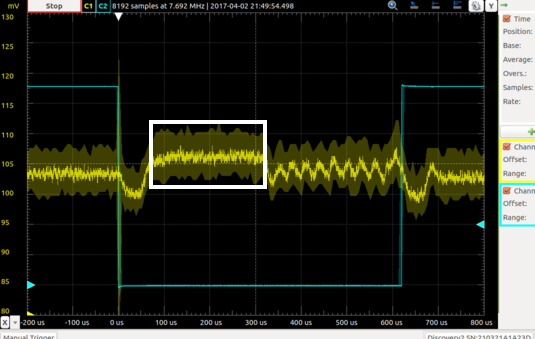
\includegraphics[scale=0.45]{aes_annotate.png}
  \caption{AES-128 capture in real-time}
  \label{fig:aes}
\end{figure}

\begin{figure}
  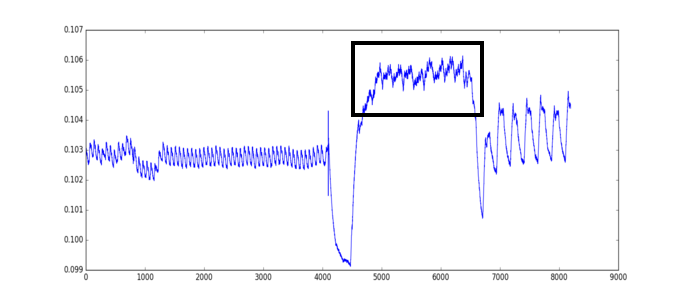
\includegraphics[scale=0.45]{aes_acquisition_annotate.png}
  \caption{AES-128 mean trace capture}
  \label{fig:aes_avg}
\end{figure}

\section{Conclusion}
Figures \ref{fig:aes} and \ref{fig:aes_avg} show that the triggering code synch up the traces well; with extra signal processing (e.g. high-pass filtering) the resulting traces should be useable for a power analysis attack.

Even though this project cannot offer concrete results, due to timing constraint, that an inexpensive piece of equipment can achieve the same result as an expensive one (i.e. enable effective power analysis attack); hopefully the theoretical points made are convincing enough to encourage further work on this topic.

\section{Appendix}
All of the code used is published on Github at the following URL: https://github.com/quangvuwpi/ECE579s

%\bibliographystyle{IEEEtran}
\bibliographystyle{IEEETR}
\bibliography{references}

\end{document}
